\documentclass[aspectratio=169, xcolor=table]{beamer}
\usetheme{TUDelft}

% ====================================================================
% ANIMATION TOGGLE
% ====================================================================
\newif\ifanimated
\animatedtrue
\ifdefined\staticmode
  \animatedfalse
\fi
\newcommand{\cpause}{\ifanimated\pause\fi}

% Import theme macros (includes TikZ libraries and semantic colors)
\usepackage{tikz}
\usetikzlibrary{positioning, shapes, arrows, shadows, fit, calc, decorations.pathreplacing}

% Semantic Colors - One meaning per color
\definecolor{irSparse}{HTML}{3498DB}   % Sparse/BM25: Blue
\definecolor{irDense}{HTML}{E67E22}    % Dense/Embeddings: Orange
\definecolor{irRerank}{HTML}{C0392B}   % Rerank/Cross-encoder: Red
\definecolor{irHybrid}{HTML}{2ECC71}   % Hybrid/Fusion: Green
\definecolor{irANN}{HTML}{9B59B6}      % ANN/Infra: Purple
\definecolor{irInfra}{HTML}{58595B}    % General Infra: Dark Gray
\definecolor{irMuted}{HTML}{D9D9D9}    % Faint Gray

% Base Styles - Consistent Diagram Grammar
\tikzset{
    irBoxBase/.style={
        rectangle, 
        draw, 
        rounded corners=2pt, 
        minimum height=0.8cm, 
        minimum width=2cm,
        font=\small\sffamily,
        align=center,
        drop shadow={opacity=0.15},
        inner sep=5pt
    },
    irDatabase/.style={
        cylinder, 
        draw, 
        shape border rotate=90, 
        aspect=0.25, 
        minimum height=1.2cm, 
        minimum width=1cm,
        fill=irMuted!20,
        draw=irInfra,
        font=\tiny\sffamily,
        align=center
    },
    % Semantic Variants
    sparse/.style={irBoxBase, fill=irSparse!10, draw=irSparse},
    dense/.style={irBoxBase, fill=irDense!10, draw=irDense},
    rerank/.style={irBoxBase, fill=irRerank!10, draw=irRerank},
    hybrid/.style={irBoxBase, fill=irHybrid!10, draw=irHybrid},
    ann/.style={irBoxBase, fill=irANN!10, draw=irANN},
    infra/.style={irBoxBase, fill=irInfra!10, draw=irInfra},
    % Legacy support / Utility
    muted/.style={irBoxBase, fill=irMuted!20, draw=irMuted!80!black, text=irMuted!50!black},
    ghost/.style={irBoxBase, fill=white, draw=irMuted!50, text=irMuted, dashed, drop shadow={opacity=0}},
    emph/.style={draw=irRerank, thick, drop shadow={shadow xshift=0mm, shadow yshift=0mm, fill=irRerank, opacity=0.3}},
    % Arrows
    irArrowBase/.style={->, thick, >=latex, draw=irInfra},
    irLabel/.style={
        font=\tiny\itshape, 
        text=irInfra, 
        align=center, 
        text width=2.5cm, 
        inner sep=3pt
    }
}


% =========================================================
% Stage Badge System
% =========================================================
% \irStage{StageName}
\newcommand{\irStage}[1]{%
    \begin{tikzpicture}[remember picture, overlay]
        \node[
            anchor=north east,
            fill=irInfra!10,
            text=irInfra,
            font=\tiny\bfseries,
            inner sep=3pt,
            rounded corners=1pt,
            yshift=-0.5cm,
            xshift=-0.5cm
        ] at (current page.north east) {#1};
    \end{tikzpicture}%
}

% =========================================================
% Math Highlighting
% =========================================================
% \mathhl[color]{content}
\newcommand{\mathhl}[2][irDense!30]{%
    \colorbox{#1}{$\displaystyle #2$}%
}

% =========================================================
% Math Vectors
% =========================================================
\newcommand{\vs}{\mathbf{s}}

% =========================================================
% Core Box Primitives
% =========================================================
% \IRBox[width]{id}{at}{title}{subtitle}{variant}
% Default width chosen for lecture slides; override when needed.
% \IRBox[width]{id}{at}{title}{subtitle}{variant}[extra options]
\DeclareDocumentCommand{\IRBox}{O{3.5cm} m m m m m O{}}{%
    \node[#6, text width=#1, #7] (#2) at #3 {%
        \textbf{#4}%
        \if\relax\detokenize{#5}\relax
        \else\\[-1mm]\scriptsize #5%
        \fi
    };%
}

% \IRWideBox{id}{at}{width}{title}{subtitle}{variant}
\newcommand{\IRWideBox}[6]{%
    \node[#6, text width=#3] (#1) at #2 {%
        \textbf{#4}%
        \if\relax\detokenize{#5}\relax
        \else\\[-1mm]\scriptsize #5%
        \fi
    };%
}

% =========================================================
% Arrow Primitives
% =========================================================
% Safe default: left-to-right flow
% \IRArrow{from}{to}{label}
\newcommand{\IRArrow}[3]{%
    \draw[irArrowBase] (#1.east) -- node[irArrowLabelAbove] {#3} (#2.west);%
}

% Explicit left-to-right
% \IRArrowLR{from}{to}{label}
\newcommand{\IRArrowLR}[3]{%
    \draw[irArrowBase] (#1.east) -- node[irArrowLabelAbove] {#3} (#2.west);%
}

% Explicit top-to-bottom
% \IRArrowTB{from}{to}{label}
\newcommand{\IRArrowTB}[3]{%
    \draw[irArrowBase] (#1.south) -- node[irArrowLabelRight] {#3} (#2.north);%
}

% Fully explicit anchor-to-anchor path
% \IRArrowPath{from anchor}{to anchor}{label}
% Example: \IRArrowPath{a.east}{b.north}{score}
\newcommand{\IRArrowPath}[3]{%
    \draw[irArrowBase] (#1) -- node[irArrowLabelAbove] {#3} (#2);%
}

% Orthogonal elbow path
% \IRArrowElbow{from anchor}{to anchor}{label}
% Example: \IRArrowElbow{a.east}{b.north}{feedback}
\newcommand{\IRArrowElbow}[3]{%
    \draw[irArrowBase] (#1) -| node[irArrowLabelBox] {#3} (#2);%
}

% Slanted arrow for special cases only
% \IRArrowSlanted{from anchor}{to anchor}{label}{pos}{width}
\newcommand{\IRArrowSlanted}[5]{%
    \draw[irArrowBase] (#1) -- node[above, sloped, irLabel, pos=#4, text width=#5, fill=white, inner sep=1pt] {#3} (#2);%
}

% =========================================================
% Accent Elements
% =========================================================
% \IRBadge{at}{text}
\newcommand{\IRBadge}[2]{%
    \node[
        draw=irAccent,
        fill=irAccent!20,
        rounded corners=1pt,
        font=\tiny\bfseries,
        inner sep=2pt
    ] at #1 {#2};%
}

% =========================================================
% Grouping
% =========================================================
% \IRGroup{fit nodes}{label}{variant}
% Example: \IRGroup{(a)(b)(c)}{First-stage retrieval}{muted}
\newcommand{\IRGroup}[3]{%
    \node[
        irGroupBase,
        #3,
        fit=#1
    ] (group) {};
    \node[
        anchor=north west,
        font=\tiny\bfseries,
        #3
    ] at ([xshift=2pt,yshift=-2pt] group.north west) {#2};%
}

% =========================================================
% Domain-Specific Shapes
% =========================================================
% \IRDocStack{id}{at}{label}
\newcommand{\IRDocStack}[3]{%
    \node[irDocStack] (#1) at #2 {#3};%
}

% \IRDatabase{id}{at}{label}
\newcommand{\IRDatabase}[3]{%
    \node[irDatabase] (#1) at #2 {#3};%
}

% =========================================================
% Layout Helpers
% =========================================================
% \IRPipelineTier{id}{at}{text}{label}{variant}
\newcommand{\IRPipelineTier}[5]{%
    \IRBox{#1}{#2}{#3}{}{#5}[]
    \node[anchor=west, irLabel, xshift=0.5cm] at (#1.east) {#4};%
}

% \IRTelescopeTier{id}{at}{width}{text}{variant}
\newcommand{\IRTelescopeTier}[5]{%
    \node[
        irTelescopeBase,
        #5,
        minimum width=#3
    ] (#1) at #2 {#4};%
}

% \IRStep{id}{at}{title}{subtitle}{variant}
% Creates a numbered step badge left of a box.
\newcommand{\IRStep}[5]{%
    \node[
        circle,
        draw=irAccent,
        fill=irAccent!20,
        font=\tiny\bfseries,
        inner sep=2pt
    ] (#1_num) at #2 {#1};
    \node[
        #5,
        text width=3.5cm,
        right=1.5cm of #1_num
    ] (#1) {%
        \textbf{#3}%
        \if\relax\detokenize{#4}\relax
        \else\\[-1mm]\scriptsize #4%
        \fi
    };
    \draw[irArrowBase, thin] (#1_num.east) -- (#1.west);%
}

\usetikzlibrary{arrows.meta}

% Additional packages for this lecture
\usepackage{booktabs}
\usepackage{listings}
\usepackage[most]{tcolorbox}

% Math definitions
\newcommand{\vq}{\mathbf{q}}
\newcommand{\vp}{\mathbf{p}}
\newcommand{\vd}{\mathbf{d}}
\newcommand{\vk}{\mathbf{k}}
\newcommand{\vv}{\mathbf{v}}
\newcommand{\vx}{\mathbf{x}}
\newcommand{\vw}{\mathbf{w}}
\newcommand{\vctx}{\mathbf{c}}
\DeclareMathOperator*{\argmax}{arg\,max}
\DeclareMathOperator*{\argmin}{arg\,min}

% Legacy color mappings for extracted TikZ
\colorlet{retrieval}{irSparse}
\colorlet{prompt}{irDense}
\colorlet{gen}{irRerank}
\colorlet{ops}{irANN}
\colorlet{warn}{irInfra}

% Title information
\title[RAG Systems 2026]{Designing, Evaluating, Debugging, and Scaling RAG Systems (2026)}
\subtitle{Lecture 7: Beyond ``BM25 + GPT'' --- A Deep Dive into RAG Architecture}
\author{Avishek Anand}
\institute{Information Retrieval}
\date{\today}

\begin{document}

% Title slide
\begin{frame}
\titlepage
\end{frame}

\begin{frame}{Outline (2 hours)}
\small
\begin{enumerate}
  \item \textbf{Framing (15)}: What RAG is (and is not), core axes
  \item \textbf{Retrieval foundation (35)}: retrieval choices, chunking, reformulation
  \item \textbf{Conditioning \& prompting (30)}: context formatting, token economics
  \item \textbf{Reasoning in RAG (30)}: multi-step, ReasonIR/Search-R1 ideas, dynamic search
  \item \textbf{Evaluation (25)}: metrics, failure taxonomy
  \item \textbf{System design \& scaling (25)}: latency, cost, production architecture
\end{enumerate}

\vspace{0.5em}
\begin{tcolorbox}[colback=gray!10,colframe=gray!40,title=Assumed known (not re-taught)]
BM25/RM3/LMs, ANN (IVF+PQ/HNSW), cross-encoders, dense retrieval (DPR/ColBERT/ANCE), hybrid, BEIR/zero-shot issues.
\end{tcolorbox}
\end{frame}

% ==========================================================
\section{Part 0 --- Framing: What is RAG?}

\begin{frame}[plain]
\sectionpage
\end{frame}

\begin{frame}{What RAG Actually Is (and is not)}
\irStage{BACKGROUND}
\textbf{RAG is a compound AI system, not a single model trick or simple recipe.}

\vspace{0.8em}
\begin{columns}[T]
\begin{column}{0.6\textwidth}
\begin{itemize}
    \item \textbf{Not}: Just ``BM25 + GPT'' or simple hallucination reduction.
    \item \textbf{Is}: A pipeline of Retrieval + Conditioning + Generation.
    \item \textbf{Core Axes}: Quality, strategy, reasoning, feedback, and cost.
\end{itemize}
\end{column}
\begin{column}{0.38\textwidth}
\begin{alertblock}{Key Thesis}
\textbf{Retrieval defines the reasoning substrate.}\\
If the evidence is not retrieved, it cannot be used by the model.
\end{alertblock}
\end{column}
\end{columns}
\end{frame}

\begin{frame}{A System View: RAG as a Pipeline of Decisions}
\irStage{SYSTEM ARCHITECTURE}
\textbf{Treat each module as a component with knobs and an evaluation contract.}

\vspace{0.5em}
\begin{center}
\resizebox{0.75\textwidth}{!}{
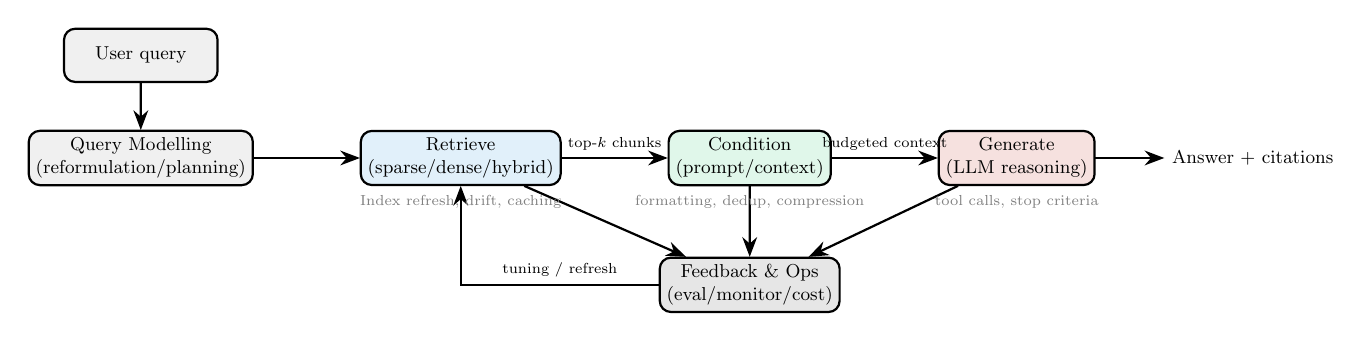
\begin{tikzpicture}[
  scale=0.75, transform shape,
  node distance=1.1cm and 1.2cm,
  box/.style={draw, rounded corners, thick, align=center, minimum height=0.9cm, minimum width=2.6cm, font=\small},
  arr/.style={-{Stealth[length=2.5mm]}, thick}
]
\node[box, fill=gray!12] (query_mod) {Query Modelling\\(reformulation/planning)};
\node[box, fill=gray!12, above=0.8cm of query_mod] (user) {User query};
\node[box, fill=irSparse!15, right=1.8cm of query_mod] (retr) {Retrieve\\(sparse/dense/hybrid)};
\node[box, fill=irHybrid!15, right=1.8cm of retr] (cond) {Condition\\(prompt/context)};
\node[box, fill=irRerank!15, right=1.8cm of cond] (gen) {Generate\\(LLM reasoning)};
\node[box, fill=irInfra!15, below=1.2cm of cond] (fb) {Feedback \& Ops\\(eval/monitor/cost)};

\draw[arr] (user) -- (query_mod);
\draw[arr] (query_mod) -- (retr);
\draw[arr] (retr) -- node[above, font=\scriptsize] {top-$k$ chunks} (cond);
\draw[arr] (cond) -- node[above, font=\scriptsize] {budgeted context} (gen);
\draw[arr] (gen) -- ++(2.5,0) node[right, font=\small] {Answer + citations};

\draw[arr] (gen) -- (fb);
\draw[arr] (retr) -- (fb);
\draw[arr] (cond) -- (fb);
\draw[arr] (fb) -| (retr) node[pos=0.25, font=\scriptsize, above] {tuning / refresh};

\node[font=\scriptsize, text=gray] at ($(retr)+(0,-0.75)$) {Index refresh, drift, caching};
\node[font=\scriptsize, text=gray] at ($(cond)+(0,-0.75)$) {formatting, dedup, compression};
\node[font=\scriptsize, text=gray] at ($(gen)+(0,-0.75)$) {tool calls, stop criteria};
\end{tikzpicture}

}
\end{center}

\cpause
\vspace{0.5em}
\begin{block}{Design Principle}
Modularity allows for isolated debugging. If generation fails, we must know if it was due to poor retrieval or poor conditioning.
\end{block}
\end{frame}

\section{Part 1 --- Retrieval: The Substrate (35 min)}

\begin{frame}[plain]
\sectionpage
\end{frame}

\begin{frame}{Retrieval Choices in RAG (2026 View)}
\irStage{RETRIEVAL}
\textbf{Choosing the right retriever depends on the trade-off between precision and OOD robustness.}

\vspace{0.8em}
\begin{table}
\centering
\resizebox{0.9\textwidth}{!}{
\begin{tabular}{l l l}
\toprule
\textbf{Method} & \textbf{Pros} & \textbf{Typical Failure} \\
\midrule
BM25 & Robust OOD, entity precision & Vocabulary mismatch \\
Dense & Semantic matching & Entity drift, OOD issues \\
Hybrid & Best practical default & Complexity, normalization \\
ColBERT & High quality at scale & Storage, infra cost \\
\bottomrule
\end{tabular}
}
\end{table}

\cpause
\vspace{0.2em}
\begin{alertblock}{The Ceiling}
\textbf{Retrieval defines the reasoning substrate.} Most ``hallucinations'' are actually \emph{selection failures}.
\end{alertblock}
\end{frame}

\begin{frame}{Retrieval Substrate: The Evidence Ceiling}
\irStage{THEORY}
\textbf{A grounded answer is a function of the query and the retrieved evidence.}

\vspace{1em}
\begin{columns}
\begin{column}{0.6\textwidth}
\[ \text{Answer}(q) = f\big(q, R_k(q)\big) \]
\cpause
\begin{itemize}
    \item If $e^\star \notin R_k(q)$, then $P(\text{correct} \mid q) \approx 0$.
    \item \textbf{Retrieve}: Find the right chunk.
    \item \textbf{Select}: Include it in context.
    \item \textbf{Use}: Force grounding via prompt.
\end{itemize}
\end{column}
\begin{column}{0.38\textwidth}
\begin{alertblock}{Debugging Mantra}
Before blaming the LLM, verify if the correct evidence was even in the prompt.
\end{alertblock}
\end{column}
\end{columns}
\end{frame}

\begin{frame}{Chunking: A Modeling Decision}
\irStage{DATA}
\textbf{Choosing the retrieval unit $u$ impacts recall, precision, and context efficiency.}

\vspace{0.8em}
\begin{columns}[T]
\begin{column}{0.5\textwidth}
\begin{itemize}
    \item \textbf{Extraction}: Tables (linearization), PDFs (layout), metadata injection.
    \item \textbf{Trade-off}: Small chunks $\uparrow$ recall, but $\downarrow$ coherence.
    \item \textbf{Standard}: Fixed-size vs. semantic chunking with overlap.
\end{itemize}
\end{column}
\begin{column}{0.48\textwidth}
\begin{center}
\resizebox{\textwidth}{!}{
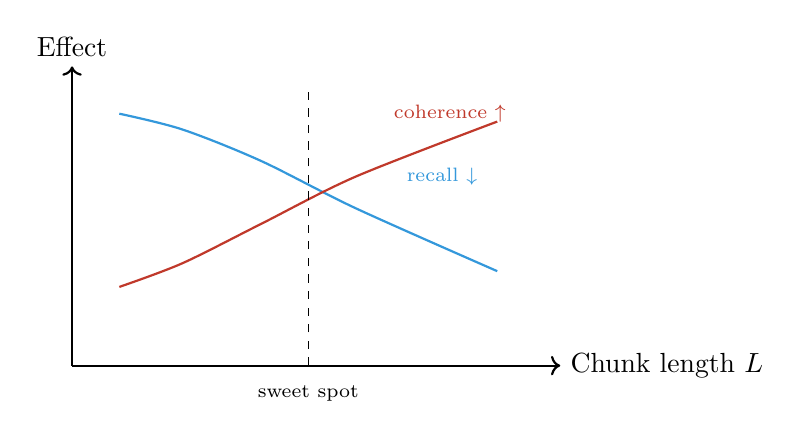
\begin{tikzpicture}[x=1cm,y=1cm]
\draw[->,thick] (0,0) -- (6.2,0) node[right] {Chunk length $L$};
\draw[->,thick] (0,0) -- (0,3.8) node[above] {Effect};
\draw[thick, irSparse] plot[smooth] coordinates {(0.6,3.2) (1.4,3.0) (2.4,2.6) (3.6,2.0) (5.4,1.2)};
\node[irSparse, font=\scriptsize] at (4.7,2.4) {recall $\downarrow$};

\draw[thick, irRerank] plot[smooth] coordinates {(0.6,1.0) (1.4,1.3) (2.4,1.8) (3.6,2.4) (5.4,3.1)};
\node[irRerank, font=\scriptsize] at (4.8,3.2) {coherence $\uparrow$};

\draw[dashed] (3.0,0) -- (3.0,3.5);
\node[font=\scriptsize] at (3.0,-0.35) {sweet spot};
\end{tikzpicture}

}
\end{center}
\end{column}
\end{columns}

\cpause
\vspace{0.5em}
\begin{block}{Rule of Thumb}
Optimize for \textbf{retrievability} and \textbf{citeability}. A chunk without source metadata effectively breaks the RAG attribution chain.
\end{block}
\end{frame}

\begin{frame}{Query Reformulation: Aligning Intent}
\irStage{RETRIEVAL}
\textbf{Bridging the lexical gap between user questions and document structure.}

\vspace{0.8em}
\begin{itemize}
    \item \textbf{HyDE}: Generate a hypothetical document to use as a semantic query.
    \item \textbf{Multi-query}: Generate diverse paraphrases to increase retrieval coverage.
    \item \textbf{Decomposition}: Break multi-part questions into sequential sub-queries.
\end{itemize}

\vspace{1em}
\cpause
\begin{alertblock}{Intent Drift}
Reformulation can shift user intent. Always monitor retrieval overlap between original and rewritten queries to detect drift.
\end{alertblock}
\end{frame}

% ==========================================================
\section{Part 2 --- Conditioning \& Prompting (30 min)}
% ==========================================================
\begin{frame}{How to Feed Retrieved Context}
\irStage{CONDITIONING}
\textbf{Context assembly impacts how well the LLM follows instructions.}

\vspace{0.3em}
\begin{columns}[T]
\begin{column}{0.52\textwidth}
\begin{block}{Context assembly strategies}
\footnotesize
\begin{itemize}
  \item Relevance-sorted + dedup + diversity
  \item Add section headers and provenance
  \item Evidence tags (\texttt{[E1]}, \texttt{[E2]}) for citations
  \item Structured formats: YAML/JSON blocks
  \item Toolformer-style search-as-tool calls
\end{itemize}
\end{block}

\cpause
\begin{alertblock}{Non-negotiable}
\footnotesize
Every chunk must carry provenance: \textbf{doc id, section, timestamp, source}.
\end{alertblock}
\end{column}

\begin{column}{0.45\textwidth}
\footnotesize
\begin{tcolorbox}[colback=gen!5,colframe=gen!50,title=Bad prompt]
\tiny
Here are some documents. Answer the question.
\end{tcolorbox}

\cpause
\vspace{0.2em}
\begin{tcolorbox}[colback=prompt!7,colframe=prompt!60,title=Good prompt]
\tiny
\textbf{Task:} Prevent speculation. Use only evidence.\\
\textbf{Input:} Question + evidence blocks \texttt{[E\#]}.\\
\textbf{Output:} Answer with citations \texttt{[E\#]}.\\
\textbf{Policy:} If evidence insufficient, say ``Insufficient evidence''.
\end{tcolorbox}
\end{column}
\end{columns}
\end{frame}

\begin{frame}[fragile]{A Practical Prompt Template (Evidence-bounded)}
\irStage{CONDITIONING}
\begin{tcolorbox}[colback=gray!8,colframe=gray!40,title=Template, fontupper=\footnotesize]
\begin{lstlisting}[basicstyle=\ttfamily\tiny]
SYSTEM: Use ONLY the evidence blocks. If insufficient, say "Insufficient evidence".
USER QUESTION: {q}
EVIDENCE:
[E1] {source=docA, section=2.1}
{chunk text...}
[E2] {source=docB, section=Table 1}
{chunk text...}
INSTRUCTIONS:
1) Answer in 3-5 bullet points.
2) Every bullet MUST cite an evidence block like [E1].
\end{lstlisting}
\end{tcolorbox}

\cpause
\vspace{-0.5em}
\begin{alertblock}{The Contract}
\footnotesize
Forcing the model to bind claims to evidence reduces hallucinations and enables automated citation verification.
\end{alertblock}
\end{frame}

\begin{frame}{Context Economics: Token Budgeting}
\irStage{SYSTEM DESIGN}
\textbf{The context window is a finite resource that must be managed to maximize reasoning quality.}

\vspace{0.8em}
\begin{columns}
\begin{column}{0.55\textwidth}
\begin{itemize}
    \item \textbf{Token Split}: System instructions, evidence, and the generated answer.
    \item \textbf{Recall vs Space}: Adding more chunks $k$ increases recall but reduces per-chunk tokens.
    \item \textbf{Best Practice}: Use a re-ranker to keep only the top-$m$ most relevant chunks.
\end{itemize}
\end{column}
\begin{column}{0.42\textwidth}
\begin{alertblock}{Budgeting Rule}
More context $\neq$ better. Wasted tokens on irrelevant chunks act as noise that degrades model performance.
\end{alertblock}
\end{column}
\end{columns}
\end{frame}

\section{Part 3 --- Reasoning: Beyond Single-Shot}

\begin{frame}[plain]
\sectionpage
\end{frame}

\begin{frame}{Reasoning: Single-shot vs Multi-step}
\irStage{REASONING}
\textbf{Complex queries often require iterative retrieval to resolve multi-hop dependencies.}

\vspace{0.5em}
\begin{columns}[T]
\begin{column}{0.48\textwidth}
\begin{itemize}
    \item \textbf{Single-shot}: Retrieve once. Fast but fails on ambiguity.
    \item \textbf{Multi-step}: Retrieve $\rightarrow$ reason $\rightarrow$ retrieve.
    \item \textbf{Requirement}: Differentiable stop criteria to control cost/latency.
\end{itemize}
\end{column}
\begin{column}{0.5\textwidth}
\begin{center}
\resizebox{\textwidth}{!}{
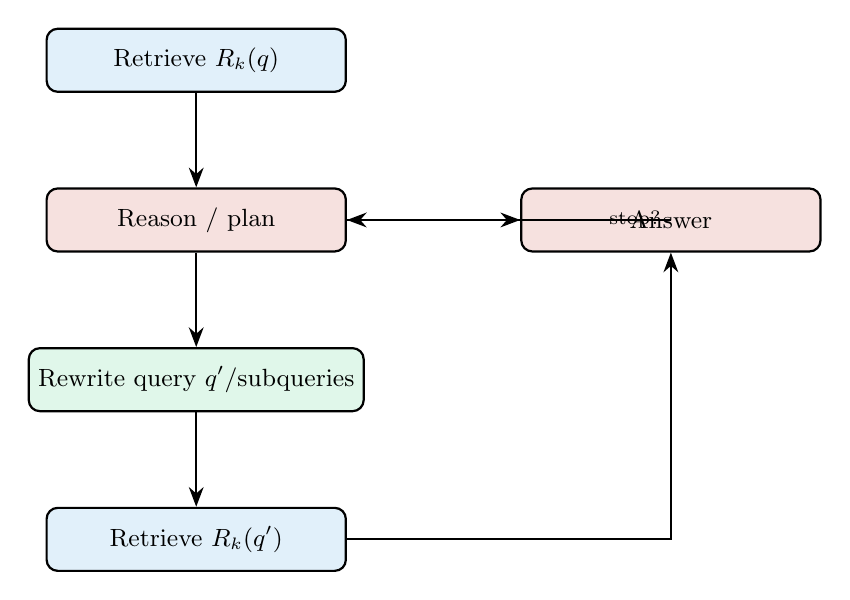
\begin{tikzpicture}[
  box/.style={draw, rounded corners, thick, align=center, font=\small, minimum width=3.8cm, minimum height=0.8cm},
  arr/.style={-{Stealth[length=2.5mm]}, thick}
]
\node[box, fill=irSparse!15] (r1) {Retrieve $R_k(q)$};
\node[box, fill=irRerank!15, below=1.2cm of r1] (think) {Reason / plan};
\node[box, fill=irHybrid!15, below=1.2cm of think] (rq) {Rewrite query $q'$/subqueries};
\node[box, fill=irSparse!15, below=1.2cm of rq] (r2) {Retrieve $R_k(q')$};
\node[box, fill=irRerank!15, right=2.2cm of think] (ans) {Answer};

\draw[arr] (r1) -- (think);
\draw[arr] (think) -- (rq);
\draw[arr] (rq) -- (r2);
\draw[arr] (r2) -| (ans);
\draw[arr] (think) -- (ans);

\draw[arr] (ans) |- (think) node[pos=0.25, font=\scriptsize, left] {stop?};
\end{tikzpicture}

}
\end{center}
\end{column}
\end{columns}
\end{frame}

\begin{frame}{Retrieval for Reasoning: Chaining Evidence}
\irStage{REASONING}
\textbf{Multi-hop questions require retrieving bridge entities that link $q$ to final $a$.}

\vspace{0.8em}
\begin{columns}[T]
\begin{column}{0.5\textwidth}
\begin{itemize}
    \item \textbf{Constraint}: Evidence $e_1$ must provide information used to find $e_2$.
    \item \textbf{Latent Links}: Bridging entities that are not explicitly in the query.
\end{itemize}
\end{column}
\begin{column}{0.48\textwidth}
\begin{center}
\resizebox{\textwidth}{!}{
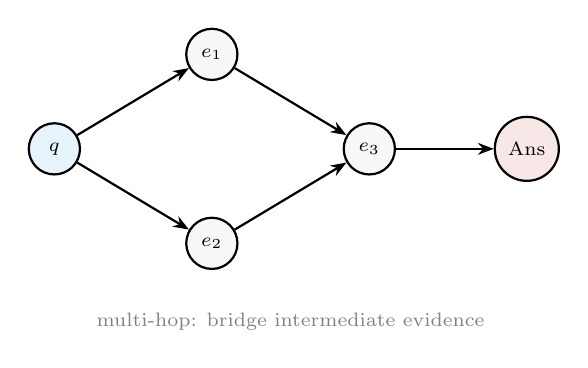
\begin{tikzpicture}[
  n/.style={draw, circle, thick, minimum size=0.65cm, font=\scriptsize},
  arr/.style={-{Stealth[length=2mm]}, thick}
]
\node[n, fill=irSparse!12] (q) at (0,0) {$q$};
\node[n, fill=irMuted!20] (e1) at (2,1.2) {$e_1$};
\node[n, fill=irMuted!20] (e2) at (2,-1.2) {$e_2$};
\node[n, fill=irMuted!20] (e3) at (4,0.0) {$e_3$};
\node[n, fill=irRerank!12] (a) at (6,0) {Ans};

\draw[arr] (q) -- (e1);
\draw[arr] (q) -- (e2);
\draw[arr] (e1) -- (e3);
\draw[arr] (e2) -- (e3);
\draw[arr] (e3) -- (a);

\node[font=\scriptsize, text=gray] at (3,-2.2) {multi-hop: bridge intermediate evidence};
\end{tikzpicture}

}
\end{center}
\end{column}
\end{columns}
\end{frame}

\begin{frame}{Search-in-the-Loop: Dynamic Retrieval}
\irStage{REASONING}
\textbf{Retrieval becomes a tool call within the LLM's reasoning trace (e.g., Search-R1).}

\vspace{0.8em}
\begin{columns}[T]
\begin{column}{0.5\textwidth}
\begin{itemize}
    \item \textbf{Trigger}: Search when model uncertainty $u_t > \theta$.
    \item \textbf{Dynamic}: Fetching new evidence only when internal knowledge is insufficient.
\end{itemize}
\end{column}
\begin{column}{0.48\textwidth}
\begin{center}
\resizebox{\textwidth}{!}{
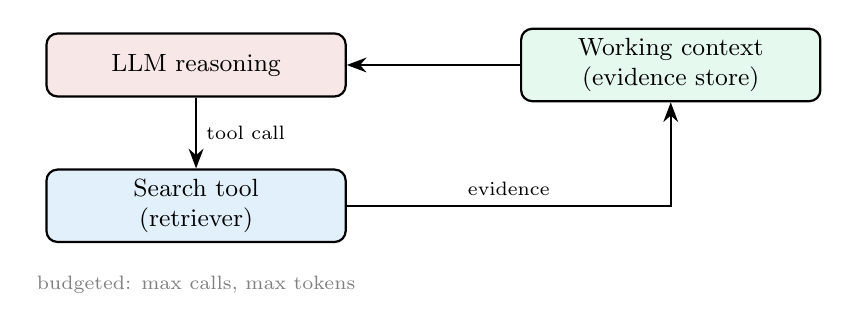
\begin{tikzpicture}[
  box/.style={draw, rounded corners, thick, align=center, font=\small, minimum width=3.8cm, minimum height=0.8cm},
  arr/.style={-{Stealth[length=2.5mm]}, thick}
]
\node[box, fill=irRerank!12] (llm) {LLM reasoning};
\node[box, fill=irSparse!15, below=0.9cm of llm] (tool) {Search tool\\(retriever)};
\node[box, fill=irHybrid!12, right=2.2cm of llm] (mem) {Working context\\(evidence store)};

\draw[arr] (llm) -- node[right, font=\scriptsize] {tool call} (tool);
\draw[arr] (tool) -| node[pos=0.25, font=\scriptsize, above] {evidence} (mem);
\draw[arr] (mem) -- (llm);

\node[font=\scriptsize, text=gray] at ($(tool)+(0,-1.0)$) {budgeted: max calls, max tokens};
\end{tikzpicture}

}
\end{center}
\end{column}
\end{columns}
\end{frame}

% ==========================================================
\section{Part 4 --- Evaluation: The RAG Triad (25 min)}

\begin{frame}[plain]
\sectionpage
\end{frame}

\begin{frame}{RAG Evaluation: Metrics \& Grounding}
\irStage{EVALUATION}
\textbf{Traditional IR metrics (Recall, nDCG) are necessary but insufficient for RAG systems.}

\vspace{0.8em}
\begin{columns}[T]
\begin{column}{0.5\textwidth}
\begin{itemize}
    \item \textbf{Faithfulness}: Is the answer supported by retrieved evidence?
    \item \textbf{Groundedness}: No extra claims beyond the evidence.
    \item \textbf{Attribution}: Do citations point to the correct supporting blocks?
\end{itemize}
\end{column}
\begin{column}{0.48\textwidth}
\begin{alertblock}{The RAG Score}
\small
\[ \text{Score} = w_1 F + w_2 A - w_3 U \]
\tiny $F$: Faithful, $A$: Attrib, $U$: Unsupported.
\footnotesize
Optimizing for correctness without attribution leads to unreliable systems.
\end{alertblock}
\end{column}
\end{columns}
\end{frame}

\begin{frame}{Failure Taxonomy: Stop Being Vague}
\irStage{EVALUATION}
\textbf{Design improvements based on specific module-level failure modes.}

\vspace{0.8em}
\begin{columns}[T]
\begin{column}{0.48\textwidth}
\begin{enumerate}
    \item \textbf{Retrieval}: $e^\star$ is missing from top-$k$.
    \item \textbf{Selection}: $e^\star$ is retrieved but dropped.
    \item \textbf{Reasoning}: $e^\star$ is misused or ignored.
    \item \textbf{Grounding}: Fabricated citations.
\end{enumerate}
\end{column}
\begin{column}{0.5\textwidth}
\begin{center}
\resizebox{\textwidth}{!}{
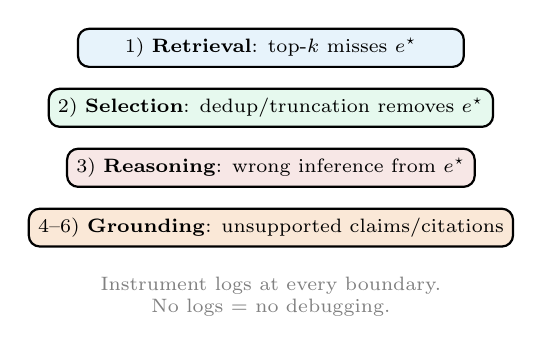
\begin{tikzpicture}[
  box/.style={draw, rounded corners, thick, align=left, font=\scriptsize, minimum width=4.9cm},
  lab/.style={font=\scriptsize, text=gray}
]
\node[box, fill=irSparse!12] (a) {1) \textbf{Retrieval}: top-$k$ misses $e^\star$};
\node[box, fill=irHybrid!12, below=0.25cm of a] (b) {2) \textbf{Selection}: dedup/truncation removes $e^\star$};
\node[box, fill=irRerank!12, below=0.25cm of b] (c) {3) \textbf{Reasoning}: wrong inference from $e^\star$};
\node[box, fill=irDense!18, below=0.25cm of c] (d) {4--6) \textbf{Grounding}: unsupported claims/citations};

\node[lab, below=0.25cm of d, align=center] {Instrument logs at every boundary.\\No logs = no debugging.};
\end{tikzpicture}

}
\end{center}
\end{column}
\end{columns}
\end{frame}

\section{Part 5 --- System Design: RAG in Production}

\begin{frame}[plain]
\sectionpage
\end{frame}

\begin{frame}{Latency Budgeting: The dominant Term}
\irStage{SYSTEM DESIGN}
\textbf{End-to-end latency is often dominated by generation tokens, not retrieval.}

\vspace{0.8em}
\begin{itemize}
    \item \textbf{Cache}: User queries and top-$k$ results for frequent intents.
    \item \textbf{Parallelize}: Run Sparse and Dense retrieval in parallel.
    \item \textbf{Early Exit}: Stop if retrieval confidence is high after re-ranking.
\end{itemize}

\vspace{1em}
\cpause
\begin{alertblock}{p95 Management}
Optimize p95 with bounded re-ranking. You cannot easily optimize LLM generation speed without reducing output token budget.
\end{alertblock}
\end{frame}

\begin{frame}{Production Architecture: The Real World}
\irStage{INFRASTRUCTURE}
\textbf{Scaling RAG requires decoupled services for retrieval and reasoning.}

\vspace{0.1em}
\begin{center}
\resizebox{0.7\textwidth}{!}{
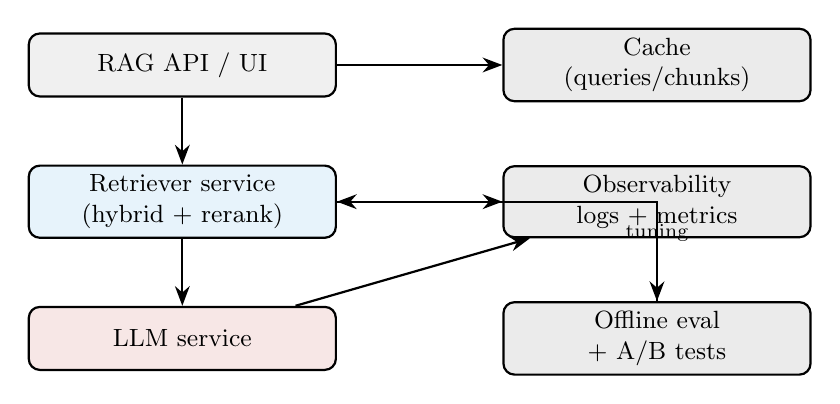
\begin{tikzpicture}[
  box/.style={draw, rounded corners, thick, align=center, font=\small, minimum width=3.9cm, minimum height=0.8cm},
  arr/.style={-{Stealth[length=2.5mm]}, thick}
]
\node[box, fill=gray!12] (api) {RAG API / UI};
\node[box, fill=irSparse!12, below=0.85cm of api] (idx) {Retriever service\\(hybrid + rerank)};
\node[box, fill=irRerank!12, below=0.85cm of idx] (llm) {LLM service};

\node[box, fill=irInfra!12, right=2.1cm of idx] (obs) {Observability\\logs + metrics};
\node[box, fill=irInfra!12, right=2.1cm of llm] (eval) {Offline eval\\+ A/B tests};
\node[box, fill=irInfra!12, right=2.1cm of api] (cache) {Cache\\(queries/chunks)};

\draw[arr] (api) -- (idx);
\draw[arr] (idx) -- (llm);

\draw[arr] (api) -- (cache);
\draw[arr] (idx) -- (obs);
\draw[arr] (llm) -- (obs);
\draw[arr] (obs) -- (eval);

\draw[arr] (eval) |- (idx) node[pos=0.25, font=\scriptsize, above] {tuning};
\end{tikzpicture}

}
\end{center}

\vspace{-0.5em}
\cpause
\begin{block}{Hard Truth}
\scriptsize
If you cannot reproduce yesterday's answer by tracing the retrieval logs, you cannot operate a production RAG system.
\end{block}
\end{frame}

\begin{frame}{Summary: The 2026 RAG Engineer}
\irStage{WRAPUP}
\textbf{RAG is a compound system of decisions across data, retrieval, and reasoning.}

\vspace{0.2em}
\begin{itemize}
    \footnotesize
    \item \textbf{Hybrid Default}: Always combine Sparse + Dense.
    \item \textbf{Metadata Chains}: Provenance must be preserved from index to prompt.
    \item \textbf{Citation Contract}: Force the model to bind claims to evidence.
    \item \textbf{Evaluation Logs}: Log retrieve $\rightarrow$ select $\rightarrow$ prompt $\rightarrow$ answer.
\end{itemize}

\vspace{0.2em}
\cpause
\begin{alertblock}{Final Takeaway}
\footnotesize
If you can't trace a claim to evidence, you don't have a RAG system --- you have a text generator.
\end{alertblock}
\end{frame}

\begin{frame}{Questions?}
\centering
\Large \textbf{Thank you!}

\vspace{2em}
\normalsize
Designing, Evaluating, Debugging, and Scaling RAG Systems (2026)
\end{frame}

\end{document}